\documentclass[11pt,a4paper]{article}

\usepackage[margin=2.2cm]{geometry}
\usepackage{tikz}
\usetikzlibrary{arrows.meta, positioning, shapes.geometric, fit, backgrounds, calc, decorations.pathreplacing}
\usepackage{xcolor}
\usepackage{titlesec}
\usepackage{enumitem}
\usepackage{amsmath}
\usepackage{amssymb}
\usepackage{booktabs}
\usepackage{longtable}
\usepackage{parskip}
\usepackage{fancyhdr}
\usepackage{hyperref}
\usepackage{tcolorbox}
\usepackage{mathtools}
\tcbuselibrary{skins,breakable}

\definecolor{navy}{HTML}{1B2A4A}
\definecolor{steel}{HTML}{2E5077}
\definecolor{teal2}{HTML}{2A9D8F}
\definecolor{amber}{HTML}{E9862F}
\definecolor{lightblue}{HTML}{DCE8F5}
\definecolor{lightgreen}{HTML}{DDEEE9}
\definecolor{lightamber}{HTML}{FBEBD9}
\definecolor{lightgrey}{HTML}{E9EBEE}

\titleformat{\part}
  {\normalfont\huge\bfseries\color{navy}}{Part \thepart}{1em}{}
\titleformat{\section}
  {\normalfont\Large\bfseries\color{navy}}{\thesection}{0.6em}{}
\titleformat{\subsection}
  {\normalfont\large\bfseries\color{steel}}{\thesubsection}{0.5em}{}
\titlespacing*{\section}{0pt}{1.4em}{0.8em}
\titlespacing*{\subsection}{0pt}{1.1em}{0.5em}

\pagestyle{fancy}
\fancyhf{}
\renewcommand{\headrulewidth}{0.4pt}
\fancyhead[L]{\small\color{steel} Indoor Drone System -- Foundations to Depth}
\fancyhead[R]{\small\color{steel} \thepage}
\renewcommand{\footrulewidth}{0pt}

\hypersetup{colorlinks=true, linkcolor=steel, urlcolor=teal2, citecolor=steel}

\tikzset{
  block/.style={rectangle, rounded corners=2pt, draw=steel, thick, fill=lightblue,
    minimum width=3.1cm, minimum height=1cm, align=center, font=\small},
  blockw/.style={block, fill=lightgreen},
  blockAmber/.style={block, fill=lightamber},
  blockGrey/.style={block, fill=lightgrey},
  decision/.style={diamond, draw=amber, thick, fill=lightamber, aspect=2.4,
    align=center, font=\scriptsize, inner sep=1pt},
  arrow/.style={-{Stealth[length=2.2mm]}, thick, steel},
  arrowd/.style={-{Stealth[length=2.2mm]}, thick, dashed, teal2},
  smallnote/.style={font=\scriptsize\itshape, color=steel!70!black},
}

\newtcolorbox{keyidea}[1][]{
  breakable, enhanced, colback=lightblue, colframe=steel,
  boxrule=0.6pt, arc=2pt, left=6pt, right=6pt, top=5pt, bottom=5pt,
  title={\textbf{Key Idea}}, fonttitle=\bfseries\color{white},
  colbacktitle=steel, #1
}
\newtcolorbox{quotebox}[1][]{
  breakable, enhanced, colback=lightamber, colframe=amber,
  boxrule=0.6pt, arc=2pt, left=6pt, right=6pt, top=5pt, bottom=5pt, #1
}
\newtcolorbox{mathbox}[1][]{
  breakable, enhanced, colback=lightgreen, colframe=teal2,
  boxrule=0.6pt, arc=2pt, left=6pt, right=6pt, top=5pt, bottom=5pt,
  title={\textbf{Math You Actually Need}}, fonttitle=\bfseries\color{white},
  colbacktitle=teal2, #1
}

\title{\vspace{-1.5cm}\textbf{\color{navy} From Zero to the Architecture}\\[4pt]
\Large\color{steel} Natural-Language-Driven Indoor Drone System\\[2pt]
\large\color{steel!70!black} A ground-up study guide -- basics, intuition, then the real math}
\author{}
\date{\small\today}

\begin{document}
\maketitle
\thispagestyle{fancy}

\begin{keyidea}[title={\textbf{How to use this document}}]
This is written assuming \textbf{zero prior knowledge} of the project. It starts from
``what is a drone'' and ``what is a coordinate'', then builds to the LLM/VLM/CV idea, and
\textbf{finally matches what is actually coded} in \texttt{Project\_phase1} today (dashboard,
code-first planner, NeLV-style stages, MATLAB UDP twin, LiteWing interface stubs for vision).
Green \textit{Math You Actually Need} boxes are equations you will tune or code. Yellow boxes
called \textbf{Codebase Reality} say what runs \emph{now} vs what is still a plan.
Read top to bottom once, then use it as notes while coding.
\end{keyidea}

\begin{quotebox}
\textbf{Codebase Reality (one paragraph).}
Today you can type natural language in the web dashboard
(\texttt{http://127.0.0.1:8000}), get a skill list, geofence-check it, and fly a MATLAB digital
twin over UDP ports 5005/5006. Simple commands (takeoff, square, go-to) use a \textbf{code
dictionary} (milliseconds). Novel commands use \textbf{Gemini}. Vision (camera $\to$ VLM
$\to$ metres) is mostly \textbf{stubbed}: FIND uses a fake bottle at $(0.5,0.5)$. Real LiteWing
hardware is wired as \texttt{--drone real} but is not the main demo yet.
\end{quotebox}

\tableofcontents

% =====================================================================
\part{Foundations}
% =====================================================================

\section{What Is a Drone, Physically?}

A \textbf{quadrotor} (4-rotor drone) is a rigid body with four spinning propellers. Each
propeller pushes air downward, which by Newton's third law pushes the drone upward. That
upward push is called \textbf{thrust}.

\begin{center}
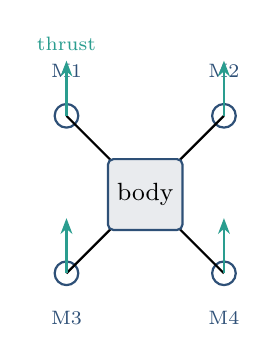
\begin{tikzpicture}
\draw[thick, steel] (0,0) circle (0.15) node[above=10pt]{\scriptsize M1};
\draw[thick, steel] (2,0) circle (0.15) node[above=10pt]{\scriptsize M2};
\draw[thick, steel] (0,-2) circle (0.15) node[below=10pt]{\scriptsize M3};
\draw[thick, steel] (2,-2) circle (0.15) node[below=10pt]{\scriptsize M4};
\draw[thick] (0,0) -- (2,-2);
\draw[thick] (2,0) -- (0,-2);
\node[blockGrey, minimum width=0.9cm, minimum height=0.9cm] at (1,-1) {body};
\draw[-{Stealth[length=2mm]}, teal2, thick] (0,0) -- (0,0.7) node[above]{\scriptsize thrust};
\draw[-{Stealth[length=2mm]}, teal2, thick] (2,0) -- (2,0.7);
\draw[-{Stealth[length=2mm]}, teal2, thick] (0,-2) -- (0,-1.3);
\draw[-{Stealth[length=2mm]}, teal2, thick] (2,-2) -- (2,-1.3);
\end{tikzpicture}
\end{center}

Each motor spins at its own speed. By making motors spin at \emph{different} speeds relative to
each other, the drone can be tilted, which redirects part of the thrust sideways -- this is how a
quadrotor moves horizontally, not by pointing a propeller sideways.

\subsection{Degrees of Freedom (DOF)}

A rigid body moving freely in 3D space has \textbf{6 degrees of freedom}: 3 for position and 3
for orientation.

\begin{center}
\small
\begin{tabular}{lll}
\toprule
\textbf{Type} & \textbf{Symbol} & \textbf{Meaning} \\
\midrule
Position & $X, Y, Z$ & location in space (metres) \\
Orientation & Roll ($\phi$) & tilt left/right, around the forward axis \\
Orientation & Pitch ($\theta$) & tilt forward/back, around the sideways axis \\
Orientation & Yaw ($\psi$) & rotation left/right, around the vertical axis \\
\bottomrule
\end{tabular}
\end{center}

For an indoor project like this one, you mostly care about $X, Y, Z$ (\emph{where} the drone is)
and yaw (\emph{which way it's facing}). Roll and pitch are used internally by the flight
controller to \emph{achieve} motion, but you as the mission designer don't command them directly
-- you command a target position, and the controller figures out the tilt needed to get there.

\begin{quotebox}
\textbf{Why this matters later:} everything in this project -- LLM, VLM, CV, homography -- exists
to answer one question, over and over: \emph{``what X, Y, Z should the drone go to next?''}
Every layer of the architecture is just narrowing that answer down from a vague human sentence to
a precise number.
\end{quotebox}

\section{What Is a Coordinate System?}

A coordinate system is just an agreed-upon way of turning ``where'' into numbers. This project
uses \textbf{two different coordinate systems} that must be connected to each other:

\begin{enumerate}[itemsep=3pt]
\item \textbf{Pixel coordinates} $(u,v)$ -- where something is in a camera image, measured in
pixels from the top-left corner.
\item \textbf{World coordinates} $(X,Y,Z)$ -- where something is in the real room, measured in
metres from a chosen origin (e.g.\ the centre of the workspace, floor level).
\end{enumerate}

\begin{center}
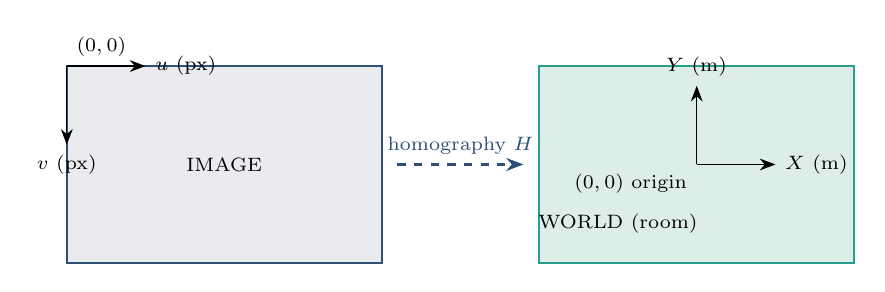
\begin{tikzpicture}
\draw[thick, steel, fill=lightgrey] (0,0) rectangle (4,-2.5);
\node[above right] at (0,0) {\scriptsize $(0,0)$};
\draw[-{Stealth[length=2mm]}] (0,0) -- (1,0) node[right]{\scriptsize $u$ (px)};
\draw[-{Stealth[length=2mm]}] (0,0) -- (0,-1) node[below]{\scriptsize $v$ (px)};
\node at (2,-1.25) {\scriptsize IMAGE};

\draw[thick, teal2, fill=lightgreen] (6,-2.5) rectangle (10,0);
\node[below left] at (8,-1.25) {\scriptsize $(0,0)$ origin};
\draw[-{Stealth[length=2mm]}] (8,-1.25) -- (9,-1.25) node[right]{\scriptsize $X$ (m)};
\draw[-{Stealth[length=2mm]}] (8,-1.25) -- (8,-0.25) node[above]{\scriptsize $Y$ (m)};
\node at (7,-2) {\scriptsize WORLD (room)};

\draw[arrow, dashed] (4.2,-1.25) -- (5.8,-1.25) node[midway, above, font=\scriptsize]{homography $H$};
\end{tikzpicture}
\end{center}

Camera pixels alone are useless to a flight controller -- a controller needs metres. The
transformation between these two systems (\textbf{homography}) is one of the mathematical cores
of this project, covered fully in Section~\ref{sec:homography}.

\section{What Is a Vector and a Matrix? (Just Enough)}

You need a minimal, practical amount of linear algebra -- not a full course.

\begin{mathbox}
A \textbf{vector} is an ordered list of numbers representing a point or direction:
\[
\mathbf{p} = \begin{pmatrix} X \\ Y \end{pmatrix}
\]
A \textbf{matrix} is a grid of numbers that \emph{transforms} vectors -- rotates them, scales
them, or moves them -- when you multiply:
\[
\mathbf{p}' = M\,\mathbf{p}
\]
For example, a 2D \textbf{rotation matrix} by angle $\theta$ is:
\[
R(\theta) = \begin{pmatrix} \cos\theta & -\sin\theta \\ \sin\theta & \cos\theta \end{pmatrix}
\]
This is exactly the kind of operation the drone's yaw and the camera's homography both use
internally: turning one set of coordinates into another via multiplication by a fixed matrix.
\end{mathbox}

\section{What Is AI, LLM, and VLM -- from Scratch}

\subsection{Machine Learning in One Paragraph}

A traditional program is written by a human: \texttt{if X then Y}. A \textbf{machine-learned}
model instead \emph{learns} a function $f$ from examples, by adjusting internal numbers
(\textbf{parameters} / \textbf{weights}) until its predictions match a huge dataset of known
answers. Once trained, you give it a new input and it produces an output using that learned
function -- no explicit rules were hand-written for that specific input.

\subsection{What Is a Large Language Model (LLM)?}

An LLM is a neural network trained on enormous amounts of text to predict \textbf{the next
token} (a token is roughly a word-piece) given the previous ones. Mathematically, at each step
it computes a probability distribution over the vocabulary:
\[
P(\text{next token} \mid \text{previous tokens})
\]
and samples (or picks the most likely) token from that distribution. Doing this repeatedly
produces a full sentence. Internally, this is powered by the \textbf{Transformer} architecture,
whose core operation is \textbf{attention} -- letting every token look at every other token and
decide how much to ``pay attention'' to it:
\[
\text{Attention}(Q,K,V) = \text{softmax}\!\left(\frac{QK^{\top}}{\sqrt{d_k}}\right)V
\]
You do \emph{not} need to implement this -- you are calling an existing LLM (Gemini, GPT, Qwen,
etc.) through an API. What matters for this project is only the \emph{input/output contract}:
you give it text (and a required output format), it gives you text back. In this project, you
design the prompt so the "text back" is structured JSON describing drone skills.

\subsection{What Is a Vision-Language Model (VLM)?}

A VLM extends the same idea to two input types at once: an image is chopped into patches,
each patch is converted into a vector (an \textbf{embedding}) the same way a word becomes a
token embedding, and the model applies attention \emph{across both the image patches and the
text tokens together}. This lets it answer questions like ``which region of this image matches
the phrase `red bottle'\,?'' The output can be structured to give you a bounding box, i.e.\ pixel
coordinates.

\begin{quotebox}
You don't need to train or fully understand a Transformer to use one well. What you \emph{do}
need to understand deeply, because you will actually design and tune it, is: prompt design,
output structure, coordinate math, and control loops. Those are covered in depth below.
\end{quotebox}

\section{What Is a Controller? (PID, from Scratch)}
\label{sec:pid}

A \textbf{controller} is the part of the system that takes a \emph{desired} value (setpoint) and
a \emph{measured} value, and computes an action to push the measured value toward the setpoint,
continuously, many times per second.

\begin{mathbox}
Define the \textbf{error} at time $t$ as the difference between where you want to be and where
you are:
\[
e(t) = x_{\text{desired}}(t) - x_{\text{measured}}(t)
\]
A \textbf{PID controller} (Proportional-Integral-Derivative) computes its output as:
\[
u(t) = \underbrace{K_p\, e(t)}_{\text{react to current error}}
+ \underbrace{K_i \int_0^t e(\tau)\,d\tau}_{\text{fix accumulated past error}}
+ \underbrace{K_d \frac{de(t)}{dt}}_{\text{dampen, predict overshoot}}
\]
\begin{itemize}[itemsep=1pt]
\item $K_p$: bigger $\to$ reacts harder to current error, but too big $\to$ oscillation.
\item $K_i$: eliminates steady-state drift (e.g.\ drone slowly sagging below hover height).
\item $K_d$: resists sudden changes, smooths the response, reduces overshoot.
\end{itemize}
$u(t)$ then feeds into \textbf{motor mixing} -- translating a desired thrust/torque into
individual motor speeds -- and finally into the physical motors.
\end{mathbox}

This is why Section 1's separation matters: an LLM cannot run this loop. $e(t)$ must be
recomputed hundreds of times per second from an IMU (inertial measurement unit) reading a
gyroscope and accelerometer at high frequency; an LLM API call can take seconds. The LLM's job
ends at producing a \emph{setpoint} ($x_{\text{desired}}$); the PID loop's job is getting there.

% =====================================================================
\part{The System, Built Up Piece by Piece}
% =====================================================================

\section{The Problem, Restated Simply}

You want to type or say:

\begin{quotebox}
\centering \Large ``Go to the red bottle.''
\end{quotebox}

...and have a real quadrotor fly to the physical location of a real red bottle, in a room, using
a fixed overhead camera to see the room -- and if the bottle moves, the drone should notice and
follow it.

That single sentence has to pass through five very different kinds of computation before it
becomes a motor command:

\begin{center}
\small
\begin{tabular}{lll}
\toprule
\textbf{Step} & \textbf{Kind of computation} & \textbf{Output} \\
\midrule
1. Understand the sentence & Language reasoning (LLM) & \texttt{FIND(red\_bottle)} \\
2. Find the object visually & Vision (CV, optionally VLM) & pixel box $[u_1,v_1,u_2,v_2]$ \\
3. Convert pixels to metres & Geometry (homography) & $(X,Y)$ in metres \\
4. Decide the next action & Planning \& safety logic & \texttt{MOVE\_TO(X,Y,Z)} \\
5. Actually fly there & Control theory (PID) & motor speeds \\
\bottomrule
\end{tabular}
\end{center}

The rest of this document builds each of those five steps in depth, then shows how they connect
into one closed loop.

\section{Step 1 -- The LLM Layer (Language $\to$ Structured Goal)}

\subsection{Why not let the LLM output motor speeds directly?}
Because of everything in Section~\ref{sec:pid}: the LLM is slow (API latency, often
hundreds of milliseconds to seconds), non-deterministic (same prompt can give slightly different
output), and has no physical model of the drone's mass, thrust curve, or current tilt. A PID loop
needs deterministic, high-frequency, physically-grounded numbers. So the LLM is only allowed to
output a \textbf{high-level goal}, not a motor value.

\begin{center}
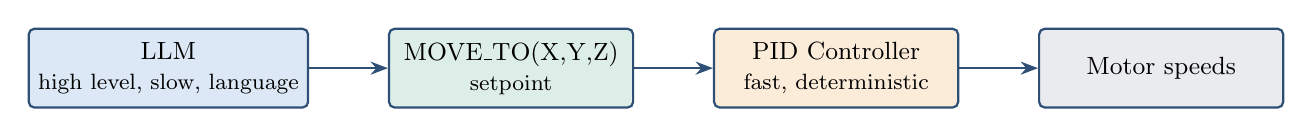
\begin{tikzpicture}[node distance=10mm]
\node[block] (llmnode) {LLM \\ \footnotesize high level, slow, language};
\node[blockw, right=of llmnode] (moveto) {MOVE\_TO(X,Y,Z) \\ \footnotesize setpoint};
\node[blockAmber, right=of moveto] (ctrl) {PID Controller \\ \footnotesize fast, deterministic};
\node[blockGrey, right=of ctrl] (motors) {Motor speeds};
\draw[arrow] (llmnode) -- (moveto);
\draw[arrow] (moveto) -- (ctrl);
\draw[arrow] (ctrl) -- (motors);
\end{tikzpicture}
\end{center}

\subsection{Skill DSL -- constraining what the LLM is allowed to say}
DSL = Domain-Specific Language. Instead of letting the LLM produce arbitrary text, the prompt
forces it to choose only from a fixed vocabulary of \textbf{skills}:
\texttt{TAKEOFF, LAND, HOVER, MOVE\_TO, ROTATE, CIRCLE, FIND, INSPECT, RETURN}, each with typed
parameters, e.g.\ \texttt{MOVE\_TO(x: float, y: float, z: float)}.

\begin{quotebox}
\textbf{Practical instruction:} in the API call you send to the LLM, instruct it to return
\emph{only} JSON matching a schema, nothing else. Then in your code, \texttt{json.loads()} the
response and validate every field against the DSL before doing anything with it. If a field is
missing, out of range, or an unknown skill name appears, reject the plan and either ask again or
fall back to a safe default (e.g.\ HOVER).
\end{quotebox}

Example prompt-to-output:
\begin{verbatim}
User: "Take off, fly to the red bottle, circle it, and land."

LLM output (structured JSON):
{
  "skills": [
    {"skill": "TAKEOFF", "params": {"z": 1.0}},
    {"skill": "FIND", "params": {"target": "red_bottle"}},
    {"skill": "CIRCLE", "params": {"target": "red_bottle", "radius": 0.5}},
    {"skill": "LAND", "params": {}}
  ]
}
\end{verbatim}

Note that \texttt{FIND} does not yet contain a coordinate -- the LLM does not know where the
bottle is. That is resolved by the next layer.

\begin{quotebox}
\textbf{Codebase Reality -- how planning actually works today}
(\texttt{backend/models/gemini\_provider.py}).
The system does \emph{not} call Gemini for every sentence. Order is:
\begin{enumerate}[itemsep=2pt]
\item \textbf{Intent router} (\texttt{intent\_router.py}): regex/dictionary. Takeoff, land-only,
square/shapes, go-to with $x,y$, relative left/right, simple FIND $\to$ \texttt{[CODE]}.
\item \textbf{Disk cache} (\texttt{plan\_cache.py}): reuse a previous Gemini plan; fill new
numbers via template key (digits $\to$ \texttt{N}).
\item \textbf{Gemini LIVE}: only if code and cache miss; JSON skills via Interactions API.
\item \textbf{NeLV finalize} (\texttt{control\_platform.py}): route POIs $\to$ densify hops
$\to$ TAKEOFF/LAND sandwich $\to$ clip to workspace.
\item \textbf{SafetyValidator} then \textbf{MissionExecutor}.
\end{enumerate}
Compound sentences (``trace S then come down'', ``if visible then circle'') intentionally
\textbf{skip} the dictionary so Gemini can invent the full sequence.
\end{quotebox}

\subsection*{Worked example A -- dictionary hit (no Gemini)}
\begin{verbatim}
Command: "take off to 1m and fly in a square"
Intent:  shape, use_code=True
Skills:  TAKEOFF(z=1.0)
         MOVE_TO corners of square (closed path)
Reasoning label: [CODE] intent=shape | NeLV parser→route→path→control
Latency: milliseconds
\end{verbatim}

\subsection*{Worked example B -- must use Gemini}
\begin{verbatim}
Command: "Trace the letter S in the air then come down"
Intent:  unknown (compound: "trace","letter","then")
Skills:  Gemini invents TAKEOFF + several MOVE_TOs approximating S + LAND
Reasoning label: [Gemini LIVE gemini-3.6-flash] ... | NeLV ...
Latency: seconds (API)
\end{verbatim}

\subsection*{Worked example C -- trap (fixed)}
\begin{verbatim}
OLD BUG: "Trace S then come down" matched "come down" → only LAND {}
FIX:     land/home only if the WHOLE command is land/home.
\end{verbatim}

\section{Step 2 -- Perception: CV vs.\ VLM}

\subsection{What Computer Vision (CV) Actually Computes}

Classical CV algorithms operate on pixel data using fixed, deterministic math -- no learned
"understanding" of language is involved (though a CV pipeline may itself use a small trained
detector like YOLO). Two things matter here: \textbf{detection} and \textbf{tracking}.

\begin{mathbox}[title={\textbf{Bounding-box center (used constantly)}}]
A detector (classical color threshold, or a trained model like YOLO) outputs a rectangle
$[u_1, v_1, u_2, v_2]$ around an object. Its centre pixel is simply:
\[
u_c = \frac{u_1+u_2}{2}, \qquad v_c = \frac{v_1+v_2}{2}
\]
Example: $[520, 310, 610, 430] \Rightarrow u_c = 565,\ v_c = 370$. This single pixel
$(u_c, v_c)$ is what gets fed into the homography in Step 3.
\end{mathbox}

\begin{mathbox}[title={\textbf{Simple color-based detection (if not using a trained model)}}]
Convert the image from RGB to \textbf{HSV} (Hue, Saturation, Value) -- hue isolates "redness"
independent of lighting brightness far better than RGB does. A pixel is classified as "red" if
its hue $H$ falls in a target range:
\[
H \in [0^\circ, 10^\circ] \cup [350^\circ, 360^\circ], \quad S > S_{\min}, \quad V > V_{\min}
\]
(red wraps around $0^\circ$ on the hue wheel). The set of matching pixels is grouped into
connected regions (\textbf{connected-component analysis}); the largest region's bounding box is
the detection.
\end{mathbox}

\textbf{Tracking} means re-identifying the same object across consecutive video frames instead of
re-detecting from scratch, e.g.\ by matching the new detection closest in position to the
previous frame's box, optionally smoothed with a simple filter:
\[
\hat{x}_t = \alpha\, x_t^{\text{measured}} + (1-\alpha)\, \hat{x}_{t-1}, \qquad 0 < \alpha \le 1
\]
This is an \textbf{exponential moving average} -- it reduces jitter from noisy detections frame
to frame ($\alpha$ close to 1 trusts new measurements more; close to 0 trusts history more).

\subsection{Why VLM Exists on Top of CV}

CV is fast and precise at geometry but has no language understanding. It cannot resolve:
\emph{``the bottle used for medicine''} or \emph{``the red bottle beside the blue cube''} on its
own. A VLM receives the image and the phrase together and returns \emph{which} detected region
(or its own bounding box) matches the description -- semantic disambiguation, not geometry.

\begin{center}
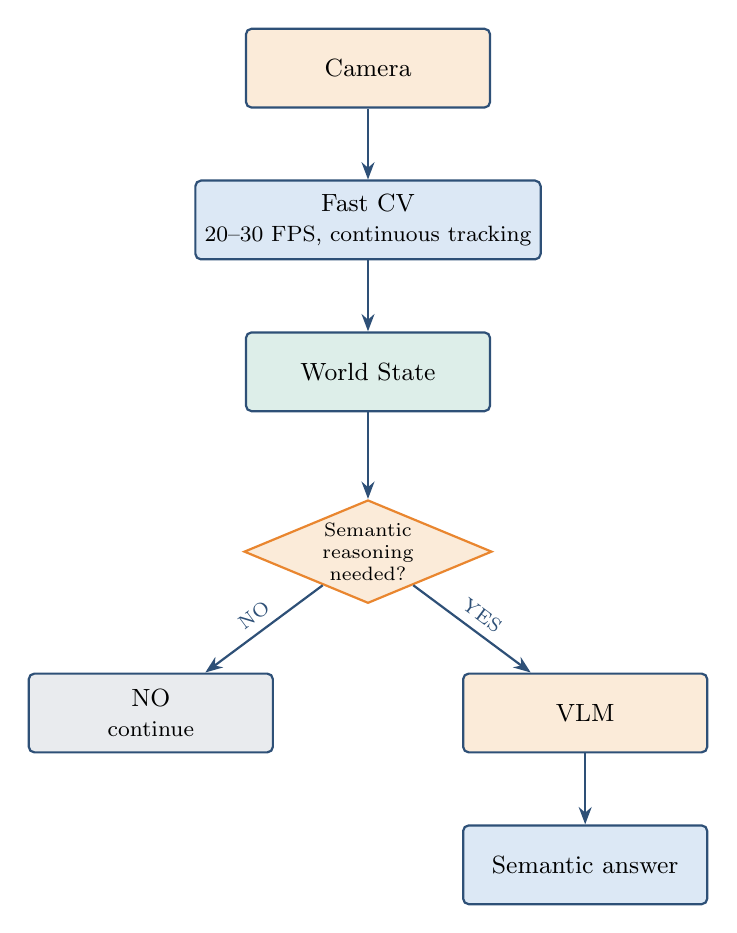
\begin{tikzpicture}[node distance=9mm]
\node[blockAmber] (cam) {Camera};
\node[block, below=of cam] (cv) {Fast CV\\ \footnotesize 20--30 FPS, continuous tracking};
\node[blockw, below=of cv] (ws) {World State};
\node[decision, below=11mm of ws, minimum width=2.6cm] (q) {Semantic\\reasoning\\needed?};
\node[blockGrey, below left=12mm and 4mm of q] (no) {NO\\ \footnotesize continue};
\node[blockAmber, below right=12mm and 4mm of q] (yes) {VLM};
\node[block, below=of yes] (sem) {Semantic answer};

\draw[arrow] (cam) -- (cv);
\draw[arrow] (cv) -- (ws);
\draw[arrow] (ws) -- (q);
\draw[arrow] (q) -- node[above, sloped, font=\scriptsize]{NO} (no);
\draw[arrow] (q) -- node[above, sloped, font=\scriptsize]{YES} (yes);
\draw[arrow] (yes) -- (sem);
\end{tikzpicture}
\end{center}

\begin{center}
\small
\begin{tabular}{ll}
\toprule
\textbf{CV} & \textbf{VLM} \\
\midrule
Fast, every frame possible & Slower, selective / event-based \\
Deterministic algorithm & Learned, probabilistic \\
Answers: \emph{where, how fast} & Answers: \emph{which one, what is it} \\
Cheap (runs locally) & Expensive (often an API call) \\
\bottomrule
\end{tabular}
\end{center}

\begin{quotebox}
\textbf{Rule of thumb:} never let the VLM output metres directly (e.g.\ ``it's at X=0.52m'').
Let it output only \emph{identity} (which object / bounding box). All coordinate math stays in
one deterministic place: the homography step. This makes errors traceable -- if a coordinate is
wrong, you know it's a geometry bug, not a hallucinated number from a generative model.
\end{quotebox}

\section{Step 3 -- From Pixels to Metres: Homography}
\label{sec:homography}

This is the mathematical heart of the perception system, so it is worth deriving properly rather
than treating as a black box.

\subsection{The Pinhole Camera Model}

A camera maps 3D world points to 2D image points via a projection. For a point lying on a
\textbf{flat plane} (e.g.\ the floor, or a table the drone flies just above), the general 3D
projection simplifies enormously to a 2D-to-2D mapping, because one dimension (height above the
plane) is fixed/known. This flat-plane assumption is exactly what makes homography usable here
instead of full 3D camera calibration.

\begin{mathbox}[title={\textbf{Homogeneous coordinates (why we add a `1')}}]
Ordinary $(X,Y)$ coordinates can represent \emph{scaling} or \emph{translation} but not both with
a single matrix multiply. The trick is to add an extra coordinate of 1:
\[
(X, Y) \ \longrightarrow\ \begin{pmatrix} X \\ Y \\ 1 \end{pmatrix}
\]
Now \emph{any} combination of rotation, scaling, shearing, and translation between two planes can
be written as a single $3\times3$ matrix multiplication. This is why homography is a
$3\times 3$ matrix, not $2\times2$.
\end{mathbox}

\begin{mathbox}[title={\textbf{The homography equation}}]
Let $(u,v)$ be a pixel and $(X,Y)$ the corresponding world point on the flat plane. Homography
says these are related, up to an unknown overall scale $s$, by a $3\times3$ matrix $H$:
\[
s\begin{pmatrix} u \\ v \\ 1 \end{pmatrix} =
H \begin{pmatrix} X \\ Y \\ 1 \end{pmatrix}
=
\begin{pmatrix} h_{11} & h_{12} & h_{13} \\ h_{21} & h_{22} & h_{23} \\ h_{31} & h_{32} & h_{33} \end{pmatrix}
\begin{pmatrix} X \\ Y \\ 1 \end{pmatrix}
\]
To use it for navigation you actually need the \textbf{inverse} direction -- pixel to world:
\[
s\begin{pmatrix} X \\ Y \\ 1 \end{pmatrix} = H^{-1} \begin{pmatrix} u \\ v \\ 1 \end{pmatrix}
\]
After the multiplication, divide the first two components by the third (this "undoes" the
unknown scale $s$ -- standard practice with homogeneous coordinates):
\[
X = \frac{X'}{s}, \qquad Y = \frac{Y'}{s} \qquad \text{where } \begin{pmatrix}X'\\Y'\\s\end{pmatrix} = H^{-1}\begin{pmatrix}u\\v\\1\end{pmatrix}
\]
\end{mathbox}

\subsection{Solving for $H$: Calibration With ArUco Markers}

$H$ has 8 independent unknowns (9 entries, minus 1 because overall scale doesn't matter -- you
can multiply the whole matrix by any nonzero number and get the same mapping). Each known
point-correspondence $(u_i, v_i) \leftrightarrow (X_i, Y_i)$ gives 2 equations, so
\textbf{4 point correspondences} (8 equations) are enough to solve for $H$ uniquely. This is
exactly why \textbf{four} ArUco markers are placed at the four known corners of the workspace.

\begin{center}
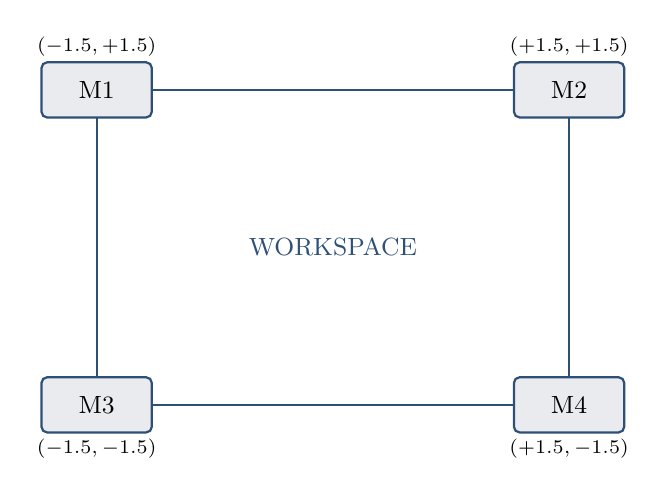
\begin{tikzpicture}
\draw[thick, steel] (0,0) rectangle (6,4);
\node[blockGrey, minimum width=1.4cm, minimum height=0.7cm] at (0,4) {M1};
\node[blockGrey, minimum width=1.4cm, minimum height=0.7cm] at (6,4) {M2};
\node[blockGrey, minimum width=1.4cm, minimum height=0.7cm] at (0,0) {M3};
\node[blockGrey, minimum width=1.4cm, minimum height=0.7cm] at (6,0) {M4};
\node[font=\small, color=steel] at (3,2) {WORKSPACE};
\node[font=\scriptsize] at (0,4.55) {$(-1.5,+1.5)$};
\node[font=\scriptsize] at (6,4.55) {$(+1.5,+1.5)$};
\node[font=\scriptsize] at (0,-0.55) {$(-1.5,-1.5)$};
\node[font=\scriptsize] at (6,-0.55) {$(+1.5,-1.5)$};
\end{tikzpicture}
\end{center}

In practice you never solve the 8 equations by hand -- OpenCV's \texttt{cv2.findHomography()}
takes the 4 pixel positions (detected automatically from the ArUco markers) and the 4 known
world positions (which you define once, by measuring your workspace), and returns $H$ using
least-squares (via \textbf{DLT}, Direct Linear Transform, if more than 4 points are given, to
average out noise). You compute $H$ \emph{once} at setup, then reuse it every frame:

\begin{verbatim}
image_pts = [[u1,v1],[u2,v2],[u3,v3],[u4,v4]]   # from ArUco detection
world_pts = [[-1.5,1.5],[1.5,1.5],[-1.5,-1.5],[1.5,-1.5]]
H, _ = cv2.findHomography(np.array(image_pts), np.array(world_pts))

# every frame, for any detected object at pixel (u,v):
world_pt = cv2.perspectiveTransform(np.array([[[u,v]]], dtype='float32'), H)
X, Y = world_pt[0][0]
\end{verbatim}

\subsection{Locating the Drone Itself}

Exactly the same math, applied to a different marker: an ArUco tag mounted on top of the drone is
detected in every frame, its centre pixel is transformed through the same $H$, giving the drone's
live $(X,Y)$. This is how the "camera never moves, drone position is always known" property is
achieved without any onboard localization hardware.

\subsection{The Z Limitation}

Homography is fundamentally a \textbf{2D-to-2D} mapping for points \emph{on the calibrated
plane}. It cannot recover height above that plane from a single overhead camera. So:
\[
\text{Camera: gives } (X, Y) \qquad \qquad \text{Flight controller: sets } Z \text{ directly (commanded altitude)}
\]
For an indoor project with a fixed target hover height, this is an acceptable simplification --
$Z$ is not perceived, it's commanded (e.g.\ "always hover at $Z=1.0$m").

\section{Step 4 -- Mission Planning and the World State}

\subsection{World State: the shared data structure}

Perception (CV + VLM) and reasoning (LLM/planner) do not talk to each other directly with raw
pixels or raw language. They share one structured object, the \textbf{World State}:

\begin{verbatim}
{
  "drone":   {"x": -0.32, "y": 0.41, "z": 1.00},
  "objects": [
    {"id": "obj_17", "label": "red_bottle", "x": 0.52, "y": 0.48, "confidence": 0.94},
    {"id": "obj_21", "label": "blue_cube",  "x": 1.10, "y": -0.30, "confidence": 0.96}
  ]
}
\end{verbatim}

This is a deliberate architectural boundary: the planner only ever reasons in metres and object
IDs, never in pixels -- which keeps it independent of camera resolution, lens, or mounting
position.

\begin{quotebox}
\textbf{Codebase Reality:} \texttt{POST /api/command} currently injects a \emph{fake} object list
(red bottle at $0.5,0.5$) into context. \texttt{FastPerception} also returns synthetic boxes.
Replace those with camera + homography before claiming vision demos.
\end{quotebox}

\subsection{Safety validation -- simple, necessary geometry checks}

Before any \texttt{MOVE\_TO(X,Y,Z)} is sent to the drone, it should be checked against hard
limits, e.g.\ a rectangular geofence:
\[
X_{\min} \le X \le X_{\max}, \qquad Y_{\min} \le Y \le Y_{\max}, \qquad Z_{\min} \le Z \le Z_{\max}
\]
and against a minimum distance to any known obstacle $(X_o, Y_o)$:
\[
\sqrt{(X - X_o)^2 + (Y - Y_o)^2} \ge d_{\text{safety}}
\]
If a proposed waypoint violates either check, it is rejected before ever reaching the flight
controller -- this is the \textbf{Safety Validator} block in the architecture diagrams.

\section{Step 5 -- Execution and Feedback}

The validated skill (e.g.\ \texttt{MOVE\_TO(0.52, 0.48, 1.0)}) is sent to a
\texttt{DroneInterface}:
\begin{itemize}[itemsep=2pt]
\item \textbf{sim} -- in-process mock (fast unit tests / UI without MATLAB).
\item \textbf{matlab} -- UDP JSON to \texttt{matlab\_udp\_bridge} (digital twin + PID).
\item \textbf{real} -- Crazyflie-style CRTP via \texttt{cflib} to LiteWing ESP32-S3.
\end{itemize}
On MATLAB/real, the low-level PID still owns attitude; Python only sends setpoints and waits
(or times out). \textbf{Camera feedback is planned}, not closed yet -- today the loop is
``plan once $\to$ execute skills'', with optional human Abort.

% =====================================================================
\part{Putting It All Together -- Matching the Codebase}
% =====================================================================

\section{What Runs Today vs.\ What Is Planned}

\begin{center}
\small
\begin{tabular}{p{4.2cm}p{5.5cm}p{5.5cm}}
\toprule
\textbf{Layer} & \textbf{Today (coded)} & \textbf{Later (VLM / hardware)} \\
\midrule
Dashboard & HTML/JS at port 8000 & same \\
NL $\to$ skills & Code + cache + Gemini & same + VLM for FIND \\
Safety & Geofence on plan & + live mid-flight abort from vision \\
Execute & Sim / MATLAB UDP / real stub & Real LiteWing CRTP flights \\
Perception & Fake objects in API context & Camera + CV + VLM + $H$ \\
Replan & FSM state unused & Target moved $\Rightarrow$ REPLAN \\
\bottomrule
\end{tabular}
\end{center}

\begin{keyidea}[title={\textbf{Memorize the honest pipeline today}}]
Dashboard $\to$ FastAPI \texttt{/api/command} $\to$ intent router (code / cache / Gemini)
$\to$ NeLV finalize (route, path, control) $\to$ SafetyValidator $\to$ MissionExecutor
$\to$ \texttt{DroneInterface} (\texttt{sim} $|$ \texttt{matlab} $|$ \texttt{real}).
Camera/VLM is \emph{not} in that path yet.
\end{keyidea}

\section{The Full Pipeline as Coded (End to End)}

\begin{center}
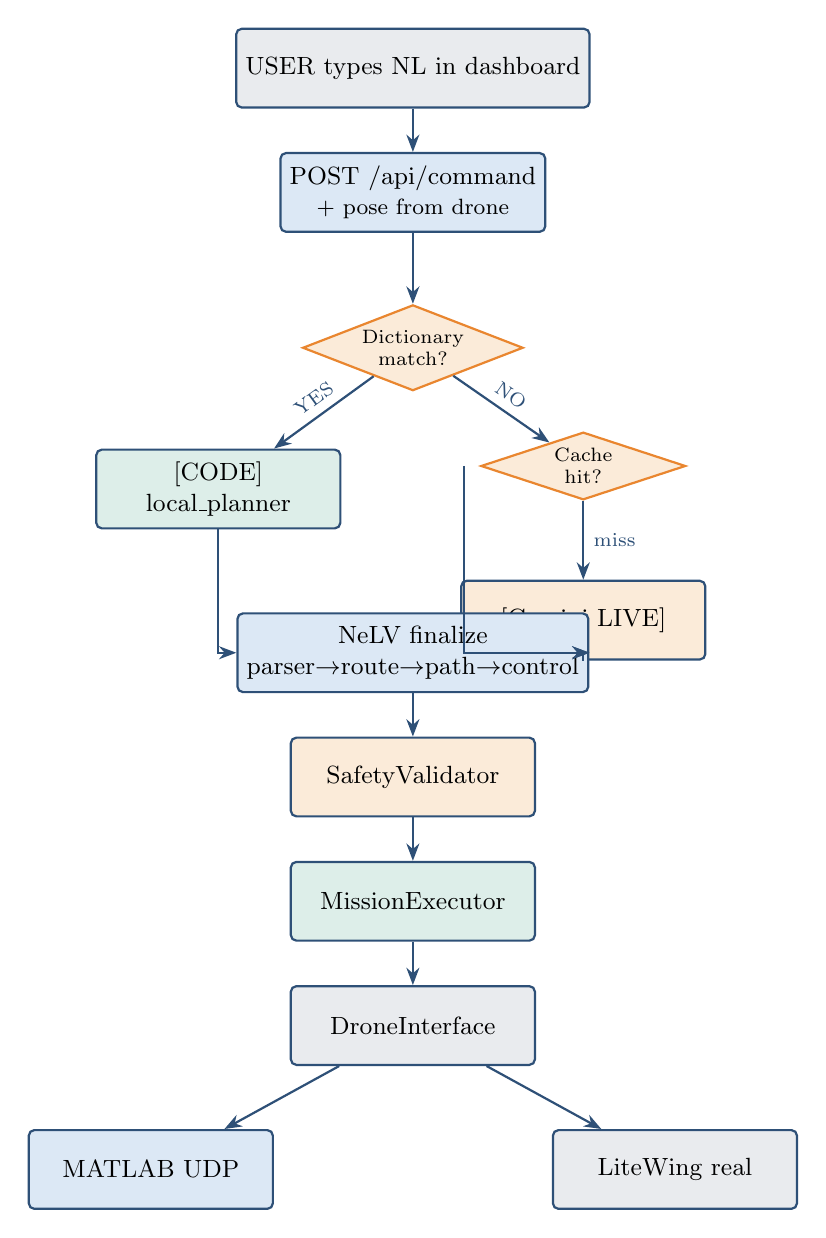
\begin{tikzpicture}[node distance=5.5mm]
\node[blockGrey] (user) {USER types NL in dashboard};
\node[block, below=of user] (api) {POST /api/command\\ \footnotesize + pose from drone};
\node[decision, below=9mm of api, minimum width=2.8cm] (code) {Dictionary\\match?};
\node[blockw, below left=10mm and 2mm of code] (local) {[CODE]\\local\_planner};
\node[decision, below right=10mm and 8mm of code, minimum width=2.6cm] (cache) {Cache\\hit?};
\node[blockAmber, below=10mm of cache] (gem) {[Gemini LIVE]};
\node[block, below=28mm of code] (nelv) {NeLV finalize\\parser$\to$route$\to$path$\to$control};
\node[blockAmber, below=of nelv] (safe) {SafetyValidator};
\node[blockw, below=of safe] (ex) {MissionExecutor};
\node[blockGrey, below=of ex] (di) {DroneInterface};
\node[block, below left=8mm and 2mm of di] (mat) {MATLAB UDP};
\node[blockGrey, below right=8mm and 2mm of di] (lw) {LiteWing real};

\draw[arrow] (user) -- (api);
\draw[arrow] (api) -- (code);
\draw[arrow] (code) -- node[above, sloped, font=\scriptsize]{YES} (local);
\draw[arrow] (code) -- node[above, sloped, font=\scriptsize]{NO} (cache);
\draw[arrow] (cache) -- node[right, font=\scriptsize]{miss} (gem);
\draw[arrow] (local) |- (nelv);
\draw[arrow] (cache.west) ++(-2mm,0) |- (nelv);
\draw[arrow] (gem) |- (nelv);
\draw[arrow] (nelv) -- (safe);
\draw[arrow] (safe) -- (ex);
\draw[arrow] (ex) -- (di);
\draw[arrow] (di) -- (mat);
\draw[arrow] (di) -- (lw);
\end{tikzpicture}
\end{center}

\subsection*{Concrete example -- square (code path)}
\begin{verbatim}
py -m backend.main --backend gemini --drone matlab
# dashboard: "take off to 1m and fly in a square"

Log:
  [CODE] intent=shape | NeLV parser→route→path→control
  TAKEOFF z=1.0
  MOVE_TO ( 0.5,  0.5, 1.0)
  MOVE_TO ( 0.5, -0.5, 1.0)
  MOVE_TO (-0.5, -0.5, 1.0)
  MOVE_TO (-0.5,  0.5, 1.0)
  MOVE_TO ( 0.5,  0.5, 1.0)   # close the loop
\end{verbatim}

Workspace clip: $X,Y \in [-1.5,1.5]$, $Z \in [0.2,1.5]$ metres
(\texttt{RobotCapabilities}).

% =====================================================================
\part{NeLV Indoor Pipeline -- A to Z}
% =====================================================================

\section{What NeLV Is (and What We Did \emph{Not} Copy)}

Outdoor research system \textbf{NeLV} (``Next-Generation LLM for UAV'')
uses five stages for large-scale missions (OSM, airports, weather). We
\textbf{borrowed the stage names and idea}, not the GIS stack.

\begin{center}
\small
\begin{tabular}{lll}
\toprule
\textbf{NeLV outdoor} & \textbf{Our indoor mapping} & \textbf{Code file} \\
\midrule
1. LLM-as-Parser & Intent + MissionSpec (metres) & \texttt{intent\_router.py} \\
2. Route Planner & POIs from known objects & \texttt{route\_planner.py} \\
3. Path Planner & Densify long MOVE\_TO hops & \texttt{path\_planner.py} \\
4. Control Platform & TAKEOFF/LAND sandwich + loiter & \texttt{control\_platform.py} \\
5. UAV Monitor & Abort + step status & \texttt{uav\_monitor.py} \\
\bottomrule
\end{tabular}
\end{center}

\begin{quotebox}
\textbf{Do not say in a viva:} ``We implemented NeLV.''\\
\textbf{Say:} ``We adapted NeLV's five-stage \emph{separation of concerns}
(parse $\neq$ fly) to a $\pm 1.5$\,m indoor geofence.''
\end{quotebox}

\section{Stage A -- Parser (Intent)}

\textbf{Job:} turn a string into a structured intent without inventing motor speeds.

\begin{center}
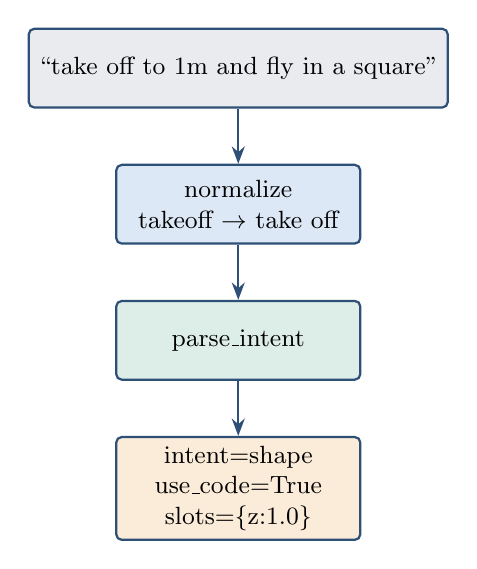
\begin{tikzpicture}[node distance=7mm]
\node[blockGrey] (in) {``take off to 1m and fly in a square''};
\node[block, below=of in] (norm) {normalize\\takeoff $\to$ take off};
\node[blockw, below=of norm] (parse) {parse\_intent};
\node[blockAmber, below=of parse] (out) {intent=shape\\use\_code=True\\slots=\{z:1.0\}};
\draw[arrow] (in)--(norm);
\draw[arrow] (norm)--(parse);
\draw[arrow] (parse)--(out);
\end{tikzpicture}
\end{center}

\textbf{Rules that matter for notes:}
\begin{itemize}[itemsep=2pt]
\item \texttt{use\_code=True} $\Rightarrow$ \texttt{local\_planner} builds skills (no Gemini).
\item Compound words (\texttt{then}, \texttt{if}, \texttt{trace}, \texttt{letter}, \ldots)
force \texttt{use\_code=False} so Gemini handles the full sentence.
\item \texttt{land}/\texttt{come down} only if the \emph{entire} command is land -- otherwise
``trace S then come down'' would wrongly become \texttt{LAND \{\}} only.
\end{itemize}

\subsection*{Examples}
\begin{center}
\small
\begin{tabular}{p{6.5cm}ll}
\toprule
\textbf{Command} & \textbf{Intent} & \textbf{Code?} \\
\midrule
\texttt{take off} & takeoff & yes \\
\texttt{take off to 1m and fly in a square} & shape & yes \\
\texttt{go to 0.3, 0.2} & goto & yes \\
\texttt{come down} & land & yes \\
\texttt{Trace the letter S then come down} & unknown & \textbf{no} $\to$ Gemini \\
\texttt{Find the red bottle. If visible...} & vision & \textbf{no} $\to$ Gemini \\
\texttt{find the red bottle} & vision & yes (template) \\
\bottomrule
\end{tabular}
\end{center}

\section{Stage B -- Route (Points of Interest)}

\textbf{Job:} decide \emph{where} in the room the mission cares about (POIs), still in metres.

Indoor ``map'' today is a tiny object table passed in API context:
\begin{verbatim}
objects = [{"label": "red_bottle", "x": 0.5, "y": 0.5, "z": 0.0},
           {"label": "blue_cube",  "x": -0.5, "y": 0.5, "z": 0.0}]
\end{verbatim}

\texttt{spec\_from\_intent} builds a \texttt{MissionSpec}: mission\_type, altitude\_m, list of
\texttt{PointOfInterest}. For FIND, it places a standoff hover near the object:
\[
x_{\text{poi}} = x_{\text{object}} - 0.35\,\text{m}, \quad y_{\text{poi}} = y_{\text{object}}
\]
Example: bottle at $(0.5,0.5)$ $\Rightarrow$ hover at $(0.15,0.5)$.

\begin{quotebox}
\textbf{Future VLM:} this stage stops reading a hardcoded table and starts reading
\texttt{WorldState} filled by camera $\to$ VLM $\to$ homography. The skill DSL stays the same.
\end{quotebox}

\section{Stage C -- Path (Waypoint Densify)}

\textbf{Job:} turn a sparse skill list into trackable hops for the plant.

If two consecutive \texttt{MOVE\_TO}s are farther than $\approx 1.05$\,m apart,
\texttt{densify\_move\_tos} inserts intermediate points so MATLAB's cascaded PID has a chance
to arrive before the 30\,s wait times out.

\begin{center}
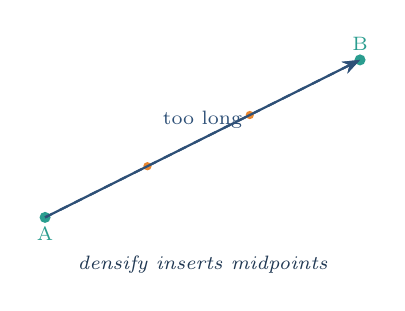
\begin{tikzpicture}
\fill[teal2] (0,0) circle (2pt) node[below]{\scriptsize A};
\fill[teal2] (4,2) circle (2pt) node[above]{\scriptsize B};
\draw[arrow, dashed] (0,0) -- (4,2) node[midway, above, font=\scriptsize]{too long};
\fill[amber] (1.3,0.65) circle (1.5pt);
\fill[amber] (2.6,1.3) circle (1.5pt);
\draw[arrow] (0,0) -- (1.3,0.65) -- (2.6,1.3) -- (4,2);
\node[smallnote] at (2,-0.6) {densify inserts midpoints};
\end{tikzpicture}
\end{center}

\section{Stage D -- Control Platform (Executable Pattern)}

\textbf{Job:} make the skill list look like a flyable mission (NeLV's takeoff/landing sandwich).

\texttt{sandwich\_takeoff\_land}:
\begin{itemize}[itemsep=2pt]
\item If mission needs air and first skill is not TAKEOFF $\Rightarrow$ prepend TAKEOFF.
\item If intent is return/land $\Rightarrow$ append LAND.
\item Optional loiter: after MOVE\_TO near a POI with \texttt{loiter\_s}, insert HOVER.
\end{itemize}

Then \texttt{clip\_skills\_to\_workspace} clamps every $x,y,z$ into the geofence.

\section{Stage E -- UAV Monitor (Operator Intervention)}

\textbf{Job:} human can stop a bad plan mid-flight.

\begin{itemize}[itemsep=2pt]
\item Dashboard \textbf{Abort} $\to$ \texttt{POST /api/abort} $\to$
\texttt{monitor.request\_abort()} + \texttt{emergency\_stop()}.
\item Executor checks \texttt{monitor.aborted()} between skills.
\item WebSocket telemetry can include \texttt{monitor} snapshot (step index, skill name).
\end{itemize}

\section{NeLV Walkthrough -- One Command, All Stages}

\textbf{Command:} \texttt{find the red bottle}

\begin{enumerate}[itemsep=3pt]
\item \textbf{Parser:} intent=\texttt{vision}, use\_code=\texttt{True}, target=\texttt{red bottle}.
\item \textbf{Local plan / route:} match object \texttt{red\_bottle} at $(0.5,0.5)$;
standoff POI $(0.15,0.5,z)$.
\item \textbf{Skills after finalize:}
\begin{verbatim}
TAKEOFF {z: 0.5}
FIND    {target: red_bottle, x: 0.15, y: 0.5, z: 0.5}
MOVE_TO {x: 0.15, y: 0.5, z: 0.5}
HOVER   {t: 2}   # loiter at POI
\end{verbatim}
\item \textbf{Path:} hops short enough -- no densify needed.
\item \textbf{Control:} TAKEOFF already present; loiter inserted.
\item \textbf{Safety:} all inside $\pm 1.5$\,m -- PASS.
\item \textbf{Execute:} FIND currently just \texttt{move\_to} (no camera yet).
\item \textbf{Monitor:} Abort still available during waits.
\end{enumerate}

\begin{quotebox}
\textbf{Honest limitation:} FIND does \emph{not} look at a camera. Visibility conditionals
(``if visible, circle; else hover'') still need Gemini for the skill list \emph{and}
a real VLM at runtime to choose the branch. Dictionary alone cannot implement true
if/else over vision.
\end{quotebox}

% =====================================================================
\part{UDP Bridge: Python $\leftrightarrow$ MATLAB}
% =====================================================================

\section{Why Two Processes?}

\begin{itemize}[itemsep=2pt]
\item \textbf{Python} = AI layer (LLM, safety, skill list, dashboard).
\item \textbf{MATLAB} = physics twin (Newton--Euler 6-DOF + cascaded PID) and optional
Simulink/Aerospace animation.
\end{itemize}
They talk with \textbf{UDP datagrams} (connectionless, low latency, JSON payloads).

\section{Port Map (Memorize)}

\begin{center}
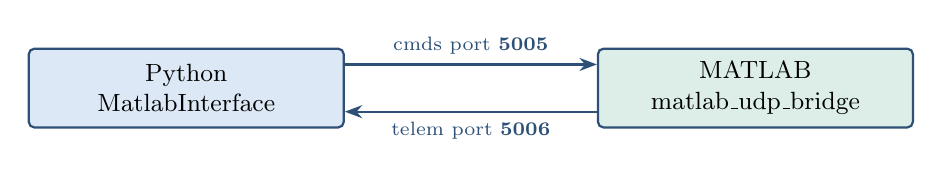
\begin{tikzpicture}
\node[block, minimum width=4cm] (py) {Python\\MatlabInterface};
\node[blockw, right=3.2cm of py, minimum width=4cm] (mat) {MATLAB\\matlab\_udp\_bridge};
\draw[arrow] ($(py.east)+(0,3mm)$) -- node[above, font=\scriptsize]{cmds port \textbf{5005}} ($(mat.west)+(0,3mm)$);
\draw[arrow] ($(mat.west)+(0,-3mm)$) -- node[below, font=\scriptsize]{telem port \textbf{5006}} ($(py.east)+(0,-3mm)$);
\end{tikzpicture}
\end{center}

\begin{center}
\small
\begin{tabular}{lll}
\toprule
\textbf{Direction} & \textbf{Port} & \textbf{Who listens} \\
\midrule
Python $\to$ MATLAB & 5005 & \texttt{matlab\_udp\_bridge.m} \\
MATLAB $\to$ Python & 5006 & \texttt{MatlabInterface} recv thread \\
\bottomrule
\end{tabular}
\end{center}

\section{Command Packet Example}

Python sends (JSON UTF-8 over UDP):
\begin{verbatim}
{"cmd": "MOVE_TO", "x": 0.5, "y": -0.5, "z": 1.0,
 "velocity": 0.5, "timestamp": 1712345678.12}
\end{verbatim}

Other \texttt{cmd} values used: \texttt{TAKEOFF}, \texttt{LAND}, \texttt{HOVER},
\texttt{ROTATE}, \texttt{EMERGENCY}, \texttt{CLEAR\_PATH}, \texttt{HOME}.

\section{Telemetry Packet Example}

MATLAB streams back (approx.\ 20\,Hz):
\begin{verbatim}
{"x":0.49,"y":-0.48,"z":0.99,"roll":2.1,"pitch":-1.3,"yaw":5.0,
 "vx":0.02,"vy":0.01,"vz":0.00,"battery_v":4.1}
\end{verbatim}

Python's \texttt{\_wait\_until\_near} polls until
\[
\sqrt{(x-x_d)^2+(y-y_d)^2+(z-z_d)^2} \le 0.08
\quad\text{and speed}\le 0.08
\]
or times out ($\sim$30\,s) and \emph{continues} (important: timeout still logs success at mission
level -- a known honesty issue for demos).

\section{How to Run the Twin (Checklist)}

\begin{enumerate}[itemsep=2pt]
\item MATLAB: \texttt{cd matlab/scripts; matlab\_udp\_bridge}
\item Python: \texttt{py -m backend.main --backend gemini --drone matlab}
\item Browser: \texttt{http://127.0.0.1:8000}
\item Optional Simulink Aerospace 6DoF Animation (manual camera/size on R2025a).
\end{enumerate}

\begin{center}
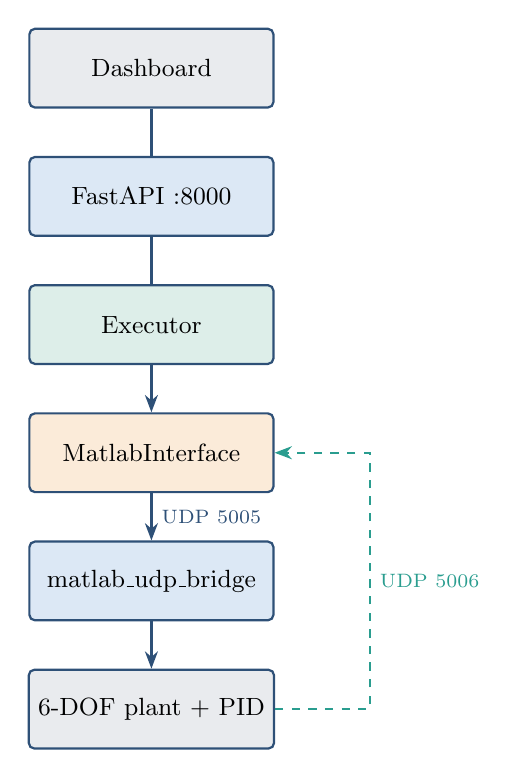
\begin{tikzpicture}[node distance=6mm]
\node[blockGrey] (dash) {Dashboard};
\node[block, below=of dash] (api) {FastAPI :8000};
\node[blockw, below=of api] (ex) {Executor};
\node[blockAmber, below=of ex] (mi) {MatlabInterface};
\node[block, below=of mi] (br) {matlab\_udp\_bridge};
\node[blockGrey, below=of br] (plant) {6-DOF plant + PID};
\draw[arrow] (dash)--(api)--(ex)--(mi);
\draw[arrow] (mi)-- node[right, font=\scriptsize]{UDP 5005} (br);
\draw[arrow] (br)--(plant);
\draw[arrowd] (plant.east) -- ++(1.2,0) |- node[near start, right, font=\scriptsize]{UDP 5006} (mi.east);
\end{tikzpicture}
\end{center}

\section{Inside the MATLAB Bridge (Plant Intuition)}

At a high level each control cycle:
\begin{enumerate}[itemsep=2pt]
\item Read latest setpoint from UDP (desired $x,y,z$).
\item Outer position / altitude controller $\to$ attitude / thrust commands.
\item Inner attitude PID $\to$ motor mixer.
\item Integrate Newton--Euler 6-DOF dynamics one timestep.
\item Publish state on 5006; optionally update live plots / Aero Animation.
\end{enumerate}

This is why MATLAB timeouts happen: if gains are soft or the hop is large, the twin never
enters the $8$\,cm ball before 30\,s -- path densify and gain tuning are the engineering fixes,
not the LLM.

% =====================================================================
\part{Controlling the Real LiteWing}
% =====================================================================

\section{DroneInterface Contract}

All backends implement the same methods
(\texttt{backend/drone/base\_interface.py}):
\texttt{connect}, \texttt{takeoff}, \texttt{land}, \texttt{hover}, \texttt{move\_to},
\texttt{rotate}, \texttt{emergency\_stop}, \texttt{get\_state}.

\begin{center}
\small
\begin{tabular}{lll}
\toprule
\textbf{Flag} & \textbf{Class} & \textbf{Transport} \\
\midrule
\texttt{--drone sim} & SimInterface & in-process mock pose \\
\texttt{--drone matlab} & MatlabInterface & UDP 5005/5006 \\
\texttt{--drone real} & LiteWingInterface & cflib CRTP UDP \\
\bottomrule
\end{tabular}
\end{center}

Default real URI in config: \texttt{udp://192.168.43.42} (phone hotspot / Wi-Fi to ESP32-S3).

\section{Command Path to Hardware (Planned / Partial)}

\begin{center}
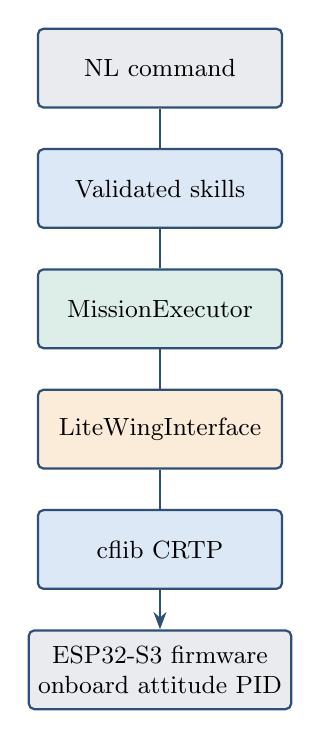
\begin{tikzpicture}[node distance=5mm]
\node[blockGrey] (nl) {NL command};
\node[block, below=of nl] (skills) {Validated skills};
\node[blockw, below=of skills] (ex) {MissionExecutor};
\node[blockAmber, below=of ex] (lw) {LiteWingInterface};
\node[block, below=of lw] (cflib) {cflib CRTP};
\node[blockGrey, below=of cflib] (esp) {ESP32-S3 firmware\\onboard attitude PID};
\draw[arrow] (nl)--(skills)--(ex)--(lw)--(cflib)--(esp);
\end{tikzpicture}
\end{center}

\textbf{Important:} high-level skills never become motor RPM in Python. The laptop sends
setpoints; the ESP32 still owns the fast attitude loop (same philosophy as MATLAB's inner PID).

\subsection*{Example sequence on hardware (same skills as sim)}
\begin{verbatim}
TAKEOFF {z: 0.8}
MOVE_TO {x: 0.4, y: 0.0, z: 0.8}
HOVER   {t: 2}
LAND    {}
\end{verbatim}
Geofence still applies -- a bad Gemini plan that asks for $z=5$\,m must be rejected or clipped
\emph{before} CRTP packets leave the laptop.

\begin{quotebox}
\textbf{Phase-1 honesty:} prove the skill DSL on MATLAB first; treat real flights as a later
acceptance test inside the same $\pm 1.5$\,m cage with a spotter and Abort bound to
\texttt{emergency\_stop}.
\end{quotebox}

% =====================================================================
\part{Future: Incorporating the VLM}
% =====================================================================

\section{Where VLM Fits (and Where It Must Not)}

\begin{center}
\small
\begin{tabular}{p{5.5cm}p{9.5cm}}
\toprule
\textbf{Allowed VLM outputs} & \textbf{Forbidden VLM outputs} \\
\midrule
Object label / which detection & Motor speeds, thrust, RPM \\
Bounding box or pixel $(u,v)$ & Hallucinated metres as ground truth \\
``visible? yes/no'' for branching & Skipping SafetyValidator \\
\bottomrule
\end{tabular}
\end{center}

\begin{keyidea}[title={\textbf{Design rule}}]
VLM answers \emph{which} and \emph{whether visible}. Homography answers \emph{where in metres}.
Code answers \emph{how to fly}. LLM/Gemini answers \emph{what skill sequence} when the dictionary
cannot.
\end{keyidea}

\section{Target Architecture After VLM}

\begin{center}
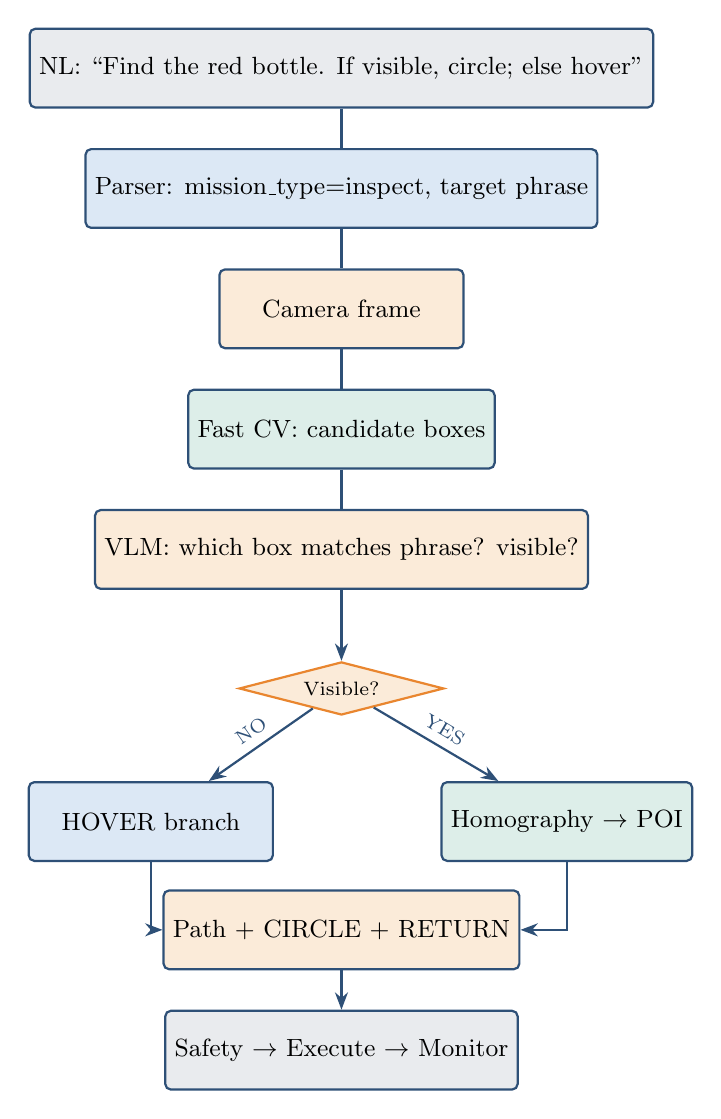
\begin{tikzpicture}[node distance=5mm]
\node[blockGrey] (nl) {NL: ``Find the red bottle. If visible, circle; else hover''};
\node[block, below=of nl] (parse) {Parser: mission\_type=inspect, target phrase};
\node[blockAmber, below=of parse] (cam) {Camera frame};
\node[blockw, below=of cam] (cv) {Fast CV: candidate boxes};
\node[blockAmber, below=of cv] (vlm) {VLM: which box matches phrase? visible?};
\node[decision, below=9mm of vlm, minimum width=2.6cm] (vis) {Visible?};
\node[block, below left=10mm and 2mm of vis] (no) {HOVER branch};
\node[blockw, below right=10mm and 6mm of vis] (yes) {Homography $\to$ POI};
\node[blockAmber, below=22mm of vis] (path) {Path + CIRCLE + RETURN};
\node[blockGrey, below=of path] (safe) {Safety $\to$ Execute $\to$ Monitor};

\draw[arrow] (nl)--(parse)--(cam)--(cv)--(vlm)--(vis);
\draw[arrow] (vis)-- node[above, sloped, font=\scriptsize]{NO} (no);
\draw[arrow] (vis)-- node[above, sloped, font=\scriptsize]{YES} (yes);
\draw[arrow] (yes)|-(path);
\draw[arrow] (no)|-(path);
\draw[arrow] (path)--(safe);
\end{tikzpicture}
\end{center}

\section{Implementation Order (Concrete)}

\begin{enumerate}[itemsep=3pt]
\item Mount overhead camera; stream frames into \texttt{CameraManager}.
\item Calibrate ArUco corners $\to$ store $H$ (homography section earlier).
\item Fast CV: detect red regions / YOLO boxes every frame $\to$ update World State.
\item Wire \texttt{GeminiProvider.resolve\_target(image, phrase)} to real multimodal Gemini
(Flash can take images) -- return bbox + label, \emph{not} metres.
\item \texttt{SpatialGrounding}: $(u_c,v_c)\xrightarrow{H}(X,Y)$; fill FIND params.
\item Only then enable conditional FIND commands and REPLAN when
$\Delta$position $> \varepsilon$.
\item Keep takeoff/square on the \textbf{code} path (do not burn VLM latency on geometry).
\end{enumerate}

\subsection*{Code touchpoints (for your notes)}
\begin{verbatim}
backend/vision/camera_manager.py     # open camera
backend/vision/fast_cv.py            # replace synthetic objects
backend/vision/spatial_grounding.py  # apply H
backend/planning/route_planner.py    # POIs from WorldState
backend/models/gemini_provider.py    # resolve_target with image bytes
backend/api/routes.py                # stop hardcoding fake bottle
backend/planning/planner.py          # use REPLANNING state
\end{verbatim}

\section{Closed-Loop Adaptive Behaviour (Target)}

If the bottle moves mid-mission, CV tracking sees jump $> \varepsilon$, perception flags
\texttt{TARGET\_CHANGED}, planner enters \texttt{REPLANNING}, route stage recomputes POI,
executor updates next \texttt{MOVE\_TO}. Re-call VLM only if identity is uncertain.

\begin{mathbox}[title={\textbf{Replan threshold}}]
\[
\sqrt{(X_t - X_{t-1})^2 + (Y_t - Y_{t-1})^2} > \varepsilon
\]
Choose $\varepsilon$ larger than stationary detection jitter.
\end{mathbox}

\section{Frequency Hierarchy}

\begin{center}
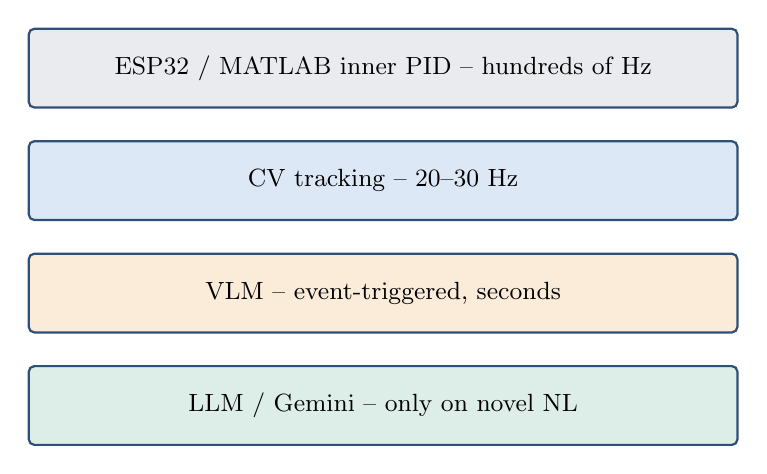
\begin{tikzpicture}[node distance=0mm]
\node[blockGrey, minimum width=9cm] (ctrl) {ESP32 / MATLAB inner PID -- hundreds of Hz};
\node[block, below=4mm of ctrl, minimum width=9cm] (cv) {CV tracking -- 20--30 Hz};
\node[blockAmber, below=4mm of cv, minimum width=9cm] (vlm) {VLM -- event-triggered, seconds};
\node[blockw, below=4mm of vlm, minimum width=9cm] (llm) {LLM / Gemini -- only on novel NL};
\end{tikzpicture}
\end{center}

\section{Why Not Simpler Architectures?}

\begin{center}
\small
\begin{tabular}{p{3.6cm}p{11.5cm}}
\toprule
\textbf{Rejected design} & \textbf{Why} \\
\midrule
CV alone (no VLM) & Cannot resolve open-vocabulary phrases. \\
LLM alone (no perception) & Names targets but never sees them. \\
VLM alone for everything & Too slow/unsafe; mixes geometry + control. \\
Gemini every takeoff & Latency; dictionary is correct for fixed skills. \\
\bottomrule
\end{tabular}
\end{center}

\section{Recommended Build Order (Aligned With Repo)}

\begin{center}
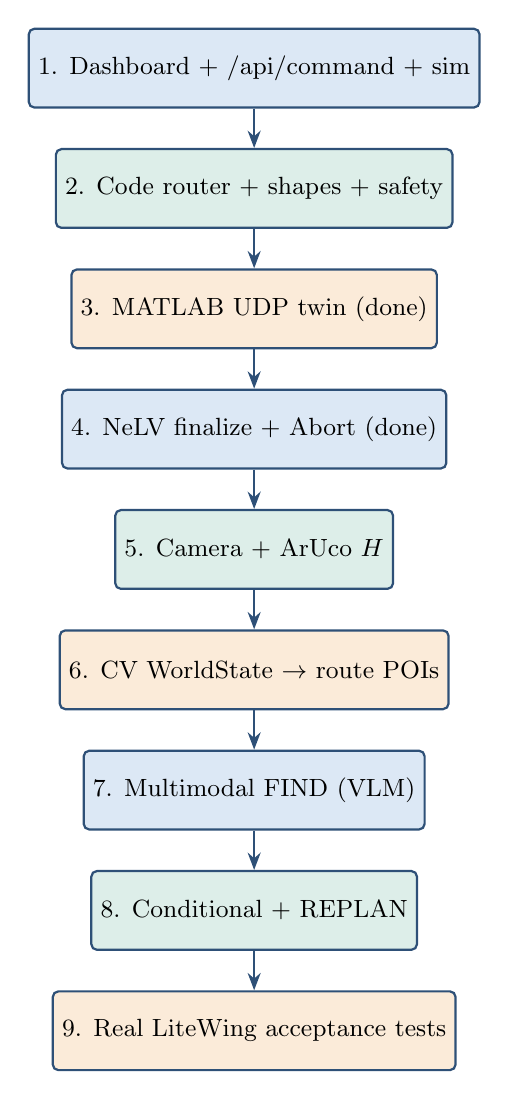
\begin{tikzpicture}[node distance=5mm]
\node[block] (s1) {1. Dashboard + /api/command + sim};
\node[blockw, below=of s1] (s2) {2. Code router + shapes + safety};
\node[blockAmber, below=of s2] (s3) {3. MATLAB UDP twin (done)};
\node[block, below=of s3] (s4) {4. NeLV finalize + Abort (done)};
\node[blockw, below=of s4] (s5) {5. Camera + ArUco $H$};
\node[blockAmber, below=of s5] (s6) {6. CV WorldState $\to$ route POIs};
\node[block, below=of s6] (s7) {7. Multimodal FIND (VLM)};
\node[blockw, below=of s7] (s8) {8. Conditional + REPLAN};
\node[blockAmber, below=of s8] (s9) {9. Real LiteWing acceptance tests};
\foreach \a/\b in {s1/s2,s2/s3,s3/s4,s4/s5,s5/s6,s6/s7,s7/s8,s8/s9}
  \draw[arrow] (\a)--(\b);
\end{tikzpicture}
\end{center}

\section{Demonstrations}

\begin{center}
\small
\begin{tabular}{p{2.2cm}p{4cm}p{8.5cm}}
\toprule
\textbf{Demo} & \textbf{Command} & \textbf{What it proves} \\
\midrule
Language / code & ``Fly in a square.'' & Dictionary + MATLAB skills \\
Novel NL & ``Trace letter S then land.'' & Gemini path (not dictionary) \\
Safety & ``Fly to 5\,m'' / go to 10,10 & Reject or refuse unsafe plans \\
Abort & Abort mid-mission & UAV Monitor \\
Vision (future) & ``Go to the red bottle.'' & VLM + $H$ + MOVE\_TO \\
Adaptive (future) & Move bottle mid-flight & REPLAN \\
\bottomrule
\end{tabular}
\end{center}

\section{One-Sentence Summaries}

\begin{keyidea}[title={\textbf{Memorize}}]
\textbf{Today:} NL $\to$ (code $|$ cache $|$ Gemini) $\to$ NeLV stages $\to$ geofence $\to$
UDP/MATLAB (or sim/real).\\
\textbf{Tomorrow:} same, but Route POIs come from camera+VLM+homography, and Monitor/REPLAN
close the loop when the world moves.\\
\textbf{Never:} let the generative model fly motors or invent metres as truth.
\end{keyidea}

\section{Viva Defence: The VLM Question}

\begin{quotebox}
\textbf{Q: ``Why VLM? Can't CV identify a red bottle?''}\\[4pt]
\textbf{A:} For fixed simple colours, CV can. We still use CV for fast tracking. VLM is for
semantic / open-vocabulary phrases (``the bottle used for medicine'', ``the red one beside the
cube'') and for visibility decisions. Once identity is known, homography gives metres.
Today FIND uses a stub pose so Phase-1 can demo language$\to$skills without a calibrated camera;
wiring the camera is the next milestone, not a claim we already have closed-loop vision.
\end{quotebox}

\begin{center}
\rule{0.4\linewidth}{0.4pt}
\end{center}
\begin{center}
\small\color{steel!70!black}
\textbf{Memorize:} LLM/code = WHAT skills $\;\bullet\;$
VLM = WHICH / visible? $\;\bullet\;$
CV = WHERE in pixels $\;\bullet\;$
Homography = WHERE in metres $\;\bullet\;$
NeLV path/control = HOW to sequence $\;\bullet\;$
Safety = ALLOWED? $\;\bullet\;$
PID (MATLAB/ESP32) = HOW TO FLY THERE $\;\bullet\;$
Monitor = HUMAN ABORT
\end{center}

\end{document}
